\chapter{剛体の力学}
\label{rigit}
細い棒を立て、ちょんと上部を押すと倒れます。この現象を力学的に見てみましょう。どのようにして運動方程式を立てれば良いでしょうか。実はこれまで扱ってきた力学は全て「質点の力学」と呼ばれるもので、物体の回転運動を考慮していませんでした。そのため、これまでの知識ではこの運動を数式化することはできません。ここでは、物体の回転運動に関して学んでいきます。

物体は全て、微小な分子に分解できます。そして、分子間の結合によってその形をとどめています。そのため、実在の物体は力をかけると変形します(この性質を持つ物体を弾性体と言います)。しかし、このような弾性体の運動を考えるには、ごくごくミクロな視点で、全ての分子に気を配らなくてはなりません。これはあまりにも大変です。

そこで、力をかけても変形しない理想的な物体である剛体を念頭に考えます。剛体であれば、一つの分子に力を加えれば、分子間の極めて硬い結合を介して、結局、全ての分子に瞬時に力が伝わります。そのため、実用上はすべての分子にいちいち気を配らなくとも物体の運動を簡単に記述できます。実在の物体は全て弾性体ですが、十分硬い物体であれば剛体に近似しても実験的事実と数式は極めて一致します。

剛体を考えるには、その剛体を構成する微小な粒子(質点)の運動方程式を考え、すべての粒子についてそれを足し合わせます。そうして「各運動量保存則」、さらにそれを用いて「回転運動方程式」を得ることができます。

\section{角運動量と力のモーメントの関係式}
\label{angularmomentum}
力学は全て運動方程式から始まります。今回求める角運動量保存則というのは、

\begin{equation}
    (角運動量の変化率) = (力のモーメント) \notag
\end{equation}

という式です。ここで、角運動量というのは物体の運動量ベクトルに左から物体の位置ベクトルを外積としてかけ合わせたものです。詳しくはこれからお話しましょう。

まずは位置ベクトル$\bm{r}$にある質量$m$の物体に力がかかるときの運動方程式を見てみましょう。

\begin{eqnarray}
    m\ddot{\bm{r}} &=& \bm{f} \notag \\
    m\frac{\mathrm{d}\bm{v}}{\mathrm{d}t} &=& \bm{f} \notag
\end{eqnarray}

ここで、後々都合が良いように$\ddot{\bm{r}}$を物体の速度$\bm{v}$の時間微分として表しました。さて、両辺に左から位置ベクトル$\bm{r}$を外積として掛け合わせてみましょう。

\begin{equation}
    \bm{r}\times\frac{\mathrm{d}\bm{v}}{\mathrm{d}t} = \bm{r}\times\bm{f} \notag
\end{equation}

ここで、左辺を都合よく変形するために、以下の式を考えてみましょう。積の微分を使って展開すると、同一な2ベクトルの外積を取る項が現れ、それは$\bm{0}$です。

\begin{eqnarray}
    \frac{\mathrm{d}}{\mathrm{d}t}\left(\bm{r}\times\bm{v}\right) &=& \frac{\mathrm{d}\bm{r}}{\mathrm{d}t}\times\bm{v}+\bm{r}\times\frac{\mathrm{d}\bm{v}}{\mathrm{d}t} \notag\\
    &=&\bm{v}\times\bm{v}+\bm{r}\times\frac{\mathrm{d}\bm{v}}{\mathrm{d}t} \notag\\
    &=&\bm{r}\times\frac{\mathrm{d}\bm{v}}{\mathrm{d}t} \notag
\end{eqnarray}

これで、先程の式は、以下のように変形できます。

\begin{eqnarray}
    \bm{r}\times\frac{\mathrm{d}\bm{v}}{\mathrm{d}t} &=& \bm{r}\times\bm{f} \notag\\
    \frac{\mathrm{d}}{\mathrm{d}t}\left(\bm{r}\times m\bm{v}\right) &=& \bm{r}\times\bm{f} \notag\\
    \frac{\mathrm{d}\bm{l}}{\mathrm{d}t} &=& \bm{n}
\end{eqnarray}

これを角運動量保存則と言い、ここで置換した$\bm{l},\bm{n}$はそれぞれ角運動量、モーメントと言います。

もう一度先程の式を出すと、この式は、

\begin{equation}
    (角運動量の変化率) = (力のモーメント) \notag
\end{equation}

という意味を持ちます。




\subsection{中心力と角運動量保存則}
\label{centralforce}
常にある一点を向いた力が物体にかかっているとしましょう。この時、この力を中心力と言います。また、力が向いている点をO(原点)とすると、物体の位置ベクトル$\bm{r}$と中心力$\bm{f}$は平行です。よって、物体に中心力のみが働くとき、

\begin{equation}
    \bm{n}=\bm{r}\times\bm{f}=\bm{0} \notag
\end{equation}

となり、$\bm{n}=\mathrm{d}\bm{l}/\mathrm{d}t$ですから、物体の角運動量は常に一定となります。つまり、中心料がはたらくときには各運動量保存則が成り立ちます。



\subsection{面積速度一定}
\label{areavelocity}
物体に中心力が働くとき、物体と力の向く先(点Oとする)を結んだ線が単位時間に掃く面積は一定になります。面積速度と角運動量の間には簡単な関係がありますので、少し確認してみましょう。

位置$\bm{r}$の点に速度$\bm{v}$で動く物体があるとき、点Oまわりの面積速度$s$は$\bm{r}$と$\bm{v}$のなす角を$\theta$として、

\begin{equation}
\label{eq:s}
    s = \frac{1}{2}rv\sin\theta
\end{equation}

となりました。ここで、角運動量の大きさ$l$は、$\bm{r}$と$\bm{v}$を2辺とする平行四辺形の面積なので、

\begin{equation}
    l = mvr\sin\theta \notag
\end{equation}

と表せます。これを式(\ref{eq:s})に代入すると、結局、

\begin{equation}
\label{eq:s2}
    s = \frac{l}{2m} \notag
\end{equation}

となります。また、面積速度はベクトル量として定義されることも多く、その定義は簡単に、

\begin{equation}
    s = \frac{1}{2}\bm{r}\times\bm{v}
\end{equation}

です。

また、\ref{centralforce}節で述べたように、物体に中心力がはたらくとき、物体の角運動量$\bm{l}$は保存されます。このときに面積速度も保存されるのは式(\ref{eq:s2})より明らかでしょう。




\section{回転運動方程式}
\label{rotationequation}
剛体の力学でよく使う、回転運動方程式を導出しましょう。これは角運動量保存則を起点として、左辺に現れる角運動量と右辺に現れるモーメントのそれぞれを剛体の場合について導出することで求められます。

\subsection{質点の角運動量}
剛体の回転運動方程式を考える前に、まずは質点の角運動量$\bm{l}$について考えます。

質点の角運動量は、

\begin{eqnarray}
    \bm{l}=\bm{r}\times m\bm{v} \notag
\end{eqnarray}

でした。ここで、$v$を$\bm{r}$に垂直な$v_\theta$と$\bm{r}$に平行な$v_r$に分解しましょう。

\begin{figure}[htbp]
\begin{center}
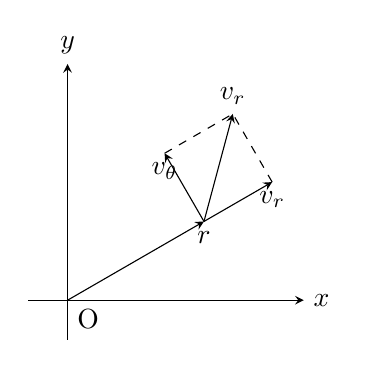
\begin{tikzpicture}[domain=-0:10,samples=300,>=stealth]
   % 座標軸
   \draw[->] (-0.5,0) -- (3,0) node[right] {$x$};
   \draw[->] (0,-0.5) -- (0,3) node[above] {$y$};
   \node [anchor=north west] at (0,0) {O};
   
   \draw[->] (0,0) -- ({2*cos(30)},{2*sin(30)}) node[below] {$\bm{r}$};
   \draw[->] ({2*cos(30)},{2*sin(30)}) -- ({2*cos(30)+sqrt(2)*cos(75)},{2*sin(30)+sqrt(2)*sin(75)}) node[above] {$\bm{v}_r$};
   \draw[->] ({2*cos(30)},{2*sin(30)}) -- ({3*cos(30)},{3*sin(30)}) node[below] {$\bm{v}_r$};
   \draw[->] ({2*cos(30)},{2*sin(30)}) -- ({2*cos(30)-cos(60)},{2*sin(30)+sin(60)}) node[below] {$\bm{v}_\theta$};
   
   \draw [dashed]({3*cos(30)},{3*sin(30)})--({2*cos(30)+sqrt(2)*cos(75)},{2*sin(30)+sqrt(2)*sin(75)});
   \draw [dashed]({2*cos(30)-cos(60)},{2*sin(30)+sin(60)})--({2*cos(30)+sqrt(2)*cos(75)},{2*sin(30)+sqrt(2)*sin(75)});
\end{tikzpicture}
\caption{$v_\theta$と$v_r$の図解}
\end{center}
\end{figure}

このとき、$v_\theta,v_r$はそれぞれ、

\begin{eqnarray}
    v_\theta=r\dot{\theta}=r\omega,\ v_r=\dot{r} \notag
\end{eqnarray}

です。$v_\theta$については、円運動の速度の式$v=r\omega$を思い出せばすぐに理解できるでしょう\footnote{これは、$x=r\cos(\omega t),y=r\sin(\omega t)$をそれぞれ$t$で微分して、$\dot{x}=-r\omega\sin(\omega t), \dot{y}=r\omega\cos(\omega t)$とし、速度ベクトルの大きさ$v=\sqrt{\dot{x}^2+\dot{y}^2}=r\omega$と導出できます。}。

そうすると、外積で算出されるベクトルの大きさは2ベクトルを2辺とする平行四辺形の面積だったので、

\begin{eqnarray}
    l=r\times mv_\theta=mr\omega^2 \notag
\end{eqnarray}

となります。

\subsection{慣性モーメント}
それでは各質点の角運動量を全部足し合わせることで、剛体の角運動量を求めましょう。剛体の角運動量の大きさ$L$は、

\begin{eqnarray}
    L=\sum_i m_ir_i^2\omega=I\omega \notag
\end{eqnarray}

となります。ここで、剛体内の全ての質点で角速度$\omega$は等しいことに注意しましょう。上の式で新たに$I$を定義しましたが、

\begin{eqnarray}
    I=\sum_i m_ir_i^2
\end{eqnarray}

を慣性モーメントと言い、その剛体の回転のしにくさを表す指標となります。

これで、角運動量保存則の左辺に現れる角運動量の、剛体の場合の式が導出できました。

\subsection{モーメント}
モーメントには質点間に働く内力によるモーメントと、外から加える外力のモーメントがあります。

結論から言うと内力のモーメントは$\bm{0}$になるのですが、それを証明しましょう。簡単のため、2質点間の内力について考えましょう。2質点間で内力が$\bm{0}$であれば、全ての質点間での内力の合計は$\bm{0}$です。

2質点(質点1、質点2)間には引力または斥力である力$\bm{f}_{12}$と$\bm{f}_{21}$が働いています。ここで、この2つの力が同じ大きさで逆向きであることを考慮すると、

\begin{eqnarray}
    \bm{n}_{12}&=&\bm{r}_1\times\bm{f}_{12}+\bm{r}_2\times\bm{f}_{21} \notag \\
    &=&\bm{r}_1\times\bm{f}_{12}-\bm{r}_2\times\bm{f}_{12} \notag \\
    &=&(\bm{r}_1-\bm{r}_2)\times\bm{f}_{12} \notag
\end{eqnarray}

ここで、$\bm{r}_1-\bm{r}_2$は$\bm{f}_{12}$に平行ですから、$\bm{n}_{12}=\bm{0}$となります。

これより、剛体を構成する各質点に働くモーメントの和は、剛体にかかる外力のモーメントに等しいことがわかります。

\subsection{回転運動方程式}

以上より、角運動量保存則の式として、

\begin{eqnarray}
    \frac{\mathrm{d}\bm{L}}{\mathrm{d}t}&=&\bm{N} \notag \\
    \frac{\mathrm{d}L}{\mathrm{d}t}&=&N \notag \\
    \frac{\mathrm{d}}{\mathrm{d}t}I\omega&=&N \notag
\end{eqnarray}

慣性モーメント$I$は物体ごとに固有で運動しても変化しないので、

\begin{eqnarray}
    I\frac{\mathrm{d}\omega}{\mathrm{d}t}&=&N
    \label{eq:rollingequation}
\end{eqnarray}

ここで、$N$は剛体にかかる力のモーメント$\bm{N}$の、回転軸に平行な成分(つまり、質点の位置ベクトル$\bm{r}$と、力ベクトル$\bm{f}$の回転軸に垂直な成分$\bm{f}_\theta$の外積の大きさ)です。

式(\ref{eq:rollingequation})を回転運動方程式と言います。

\section{回転による運動エネルギー}
回転による運動エネルギーは、各質点の運動エネルギー$1/2m_iv_i^2=1/2m_i(r_i\omega)^2$の総和ですから、

\begin{eqnarray}
    K&=&\sum_i\left(\frac{1}{2}m_i(r_i\omega)^2\right) \notag \\
    &=&\sum_i\left(\frac{1}{2}m_ir_i^2\right)\omega^2 \notag \\
    &=&\frac{1}{2}I\omega^2
\end{eqnarray}